\subsection{L1L2}

The L1L2 dataset with the SVT at the nominal 0.5~mm position consists of tracks where the one track missed the active region of Layer 1. This dataset combines the case for which the electron passes through Layer 1 and the positron passes through Layer 1 in order to obtaining the zCut because it was noted that the tails of the distributions are the same (despite the known backgrounds being different and could merit improved cuts that would divide the dataset in the future). 

\subsubsection{Cuts}

The cuts applied to the L1L2 dataset are shown in Table~\ref{l1l2_cuts}. 

\begin{table}[H]
\caption{Cuts applied to the L1L2 datasets.}
\label{l1l2_cuts}
\centering
\begin{tabular}{lllllll}
\toprule
%\multicolumn{2}{c}{Name} \\
%\cmidrule(r){1-2}
Cut type & Cut & Cut Value &  $\%$killed &  $\%$killed core & $\%$killed tails\\
\midrule
track & Fit quality & track $\chi^{2}<30$ & 38 & 15 & 47 \\
track & Max track momentum &  $P_{trk}<75\%E_{beam}$ & 12 & 8 & 14 \\
track & Isolation &   & 11 & 4 & 15 \\
vertex & beamspot constraint & bsc$\chi^{2}<10$  & 46 & 24 & 60 \\
vertex & beamspot - unconstrained & bsc$\chi^{2}$-unc$\chi^2<5$  & 20 & 16 & 24 \\
vertex & maximum $P_{sum}$ &  $<115\%E_{beam}$ & 1 & 1 & 1 \\
ecal & Ecal SVT matching & $\chi^2<10$  & 7 & 7 & 8 \\
ecal & track Ecal timing & $<4$ns  & 5 & 5 & 5 \\
ecal & 2 cluster time diff & $<2$ns  & 8 & 6 & 10 \\
physics & momentum asymmetry & $<0.4$  & 14 & 15 & 13 \\
physics & e+ track d0 & $<1.5$mm  & 7 & 3 & 11 \\
event & max shared hits amongst tracks & $<5$ shared hits  & 8 & 7 & 8 \\
track & cuts on kink tails & $\phi$ and $\lambda$ kink tails & 19 & 9 & 36 \\
\bottomrule
\end{tabular}
\end{table}

The initial selection requires that a track that missed Layer 1 has a projection to the z location at layer 1 that is less than 1.5~mm from the beam. This ensures that the sample is not overly contaminated by events that passed through the active region but failed to identify a hit. As a result, the core of the distribution sits on the downstream side of the z-axis and reflects the geometric constraints we have imposed. The first cut that is different from the L1L1 dataset is the isolation cut. In this dataset, we apply the same isolation cut to the track that passed through Layer 1, but we apply a slightly different isolation cut for the track that did not pass through layer 1. The isolation in layer 2 is measured and projected to the target position to be compared with the impact parameter of the track in y at the target. Additional cuts are applied to the tails of the kink distributions for the tracks. The summary of these cuts is made in the Table~\ref{kink_cuts}.

\begin{table}[H]
\caption{Cuts applied to the kinks in layers 1-3.}
\label{kink_cuts}
\centering
\begin{tabular}{lll}
\toprule
%\multicolumn{2}{c}{Name} \\
%\cmidrule(r){1-2}
Cut & Value \\
\midrule
Layer 1: $\phi$ kink, $\lambda$ kink & <0.0001,<0.002\\
Layer 2: $\phi$ kink, $\lambda$ kink & <0.002,<0.004\\
Layer 3: $\phi$ kink, $\lambda$ kink & <0.002,<0.004\\
\bottomrule
\end{tabular}
\end{table}

The uncut kink distributions for the electron with the cut indicated by the red dashed line is shown in Figures~\ref{fig:kink1}, \ref{fig:kink2}, and \ref{fig:kink3}.

\begin{figure}[H]
  \centering
      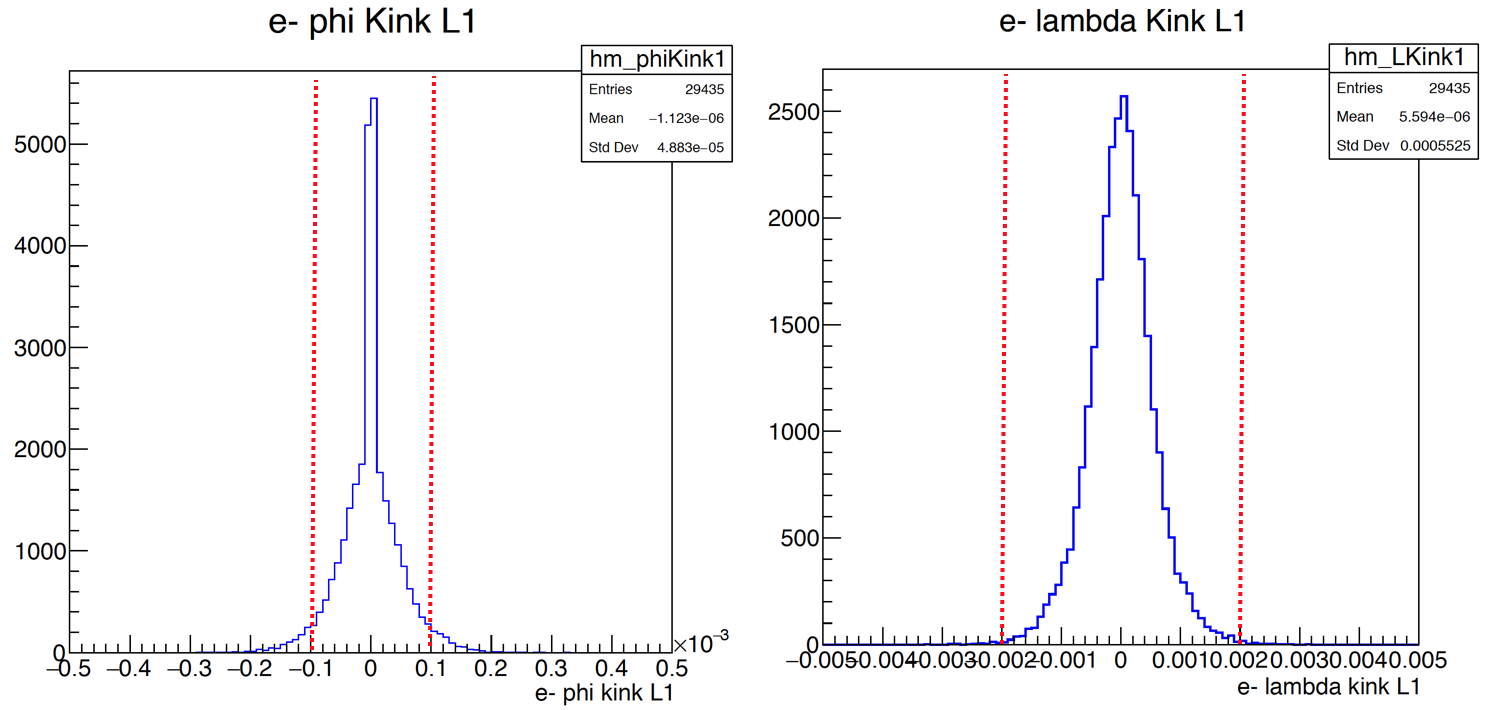
\includegraphics[width=0.8\textwidth]{plots/kink1.png}
  \caption{The kink distributions for tracks passing through Layer 1. The cut is shown at the red dashed line.}
  \label{fig:kink1}
\end{figure} 
\begin{figure}[H]
  \centering
      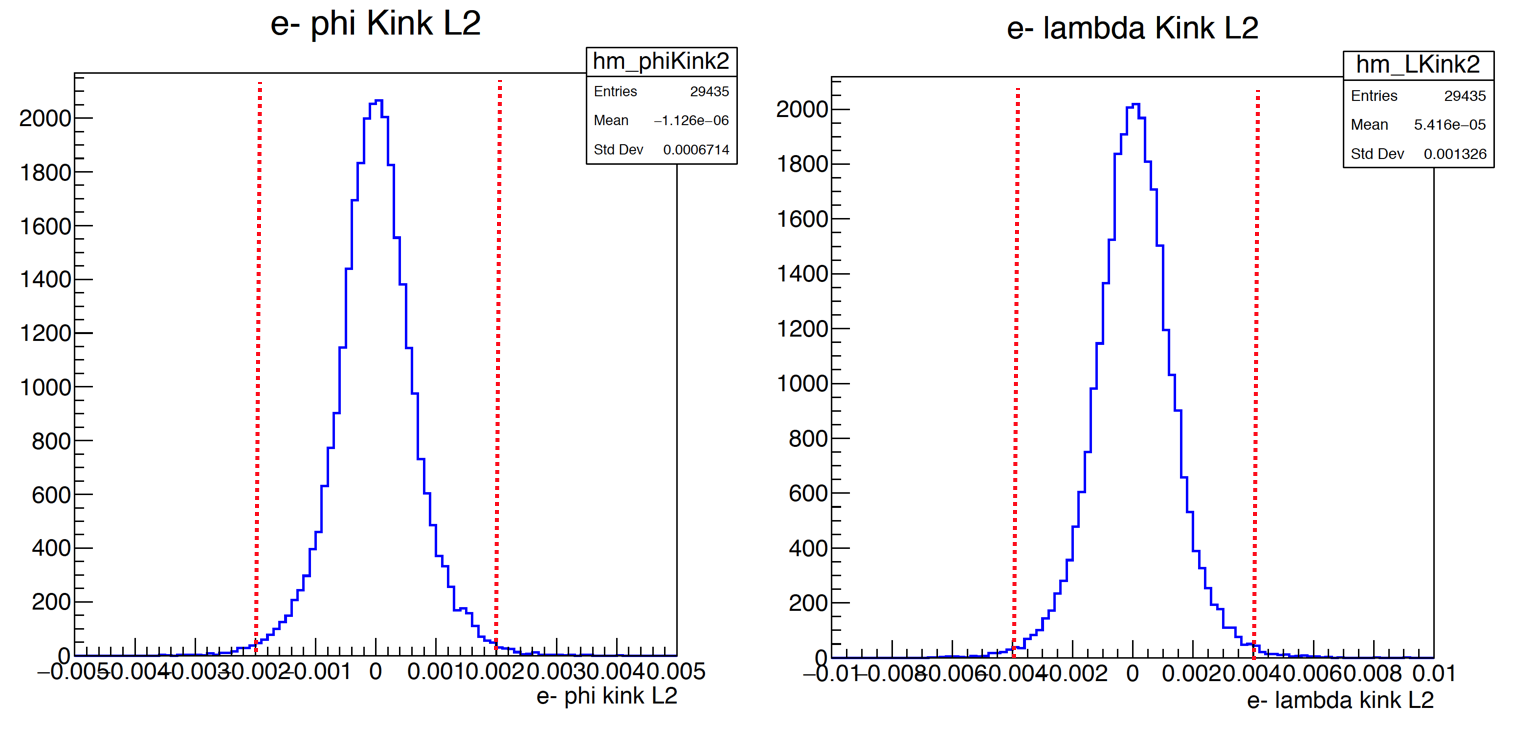
\includegraphics[width=0.8\textwidth]{plots/kink2.png}
  \caption{The kink distributions for tracks passing through Layer 2. The cut is shown at the red dashed line.}
  \label{fig:kink2}
\end{figure} 
\begin{figure}[H]
  \centering
      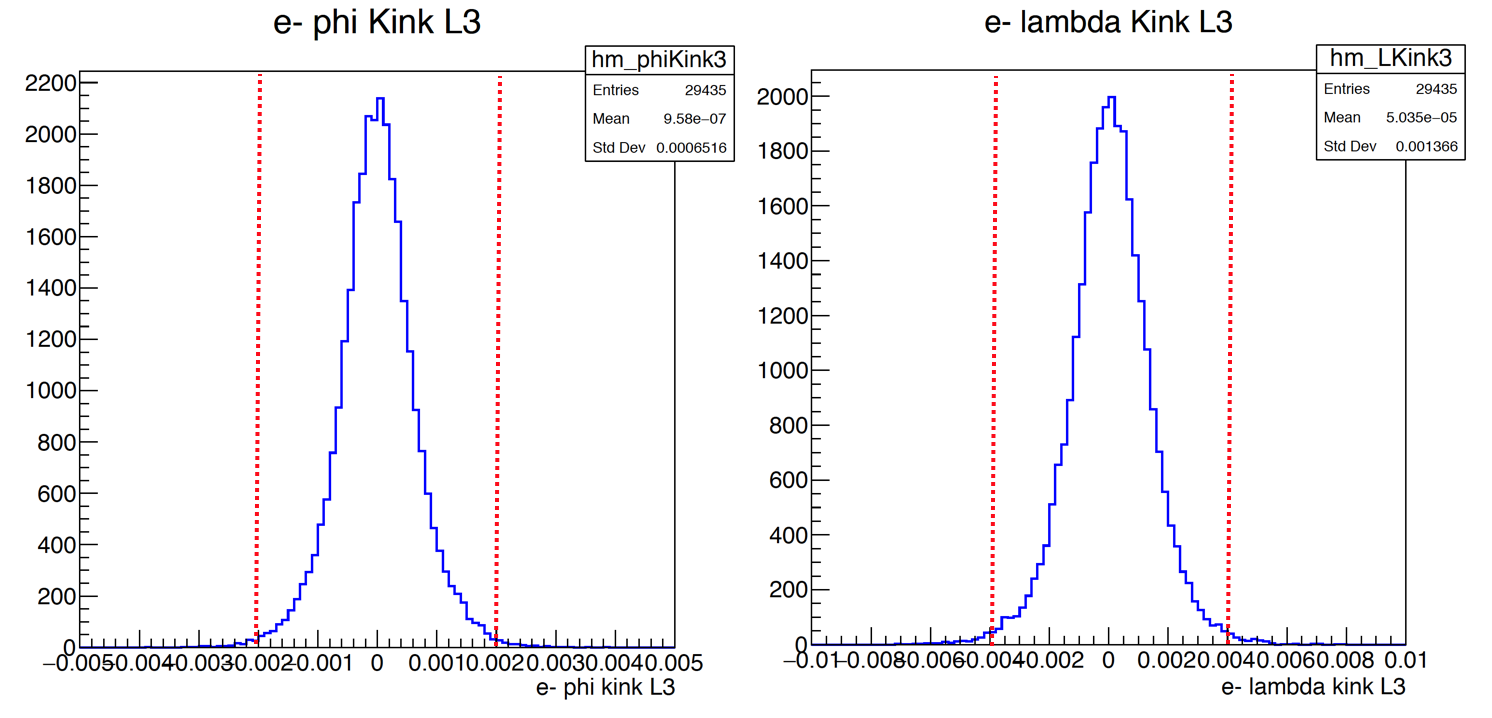
\includegraphics[width=0.8\textwidth]{plots/kink3.png}
  \caption{The kink distributions for tracks passing through Layer 3. The cut is shown at the red dashed line.}
  \label{fig:kink3}
\end{figure} 

The positron kink distributions look like the electron kink distributions are not showen here. These cuts significantly remove events from the tails and merit further study with the unblinded dataset to increase statistics in understanding cuts. The effects of all the cuts on the reconstructed vertex position distribution are shown in Figure~\ref{fig:zvtxCuts_l1l2}.

\begin{figure}[H]
  \centering
      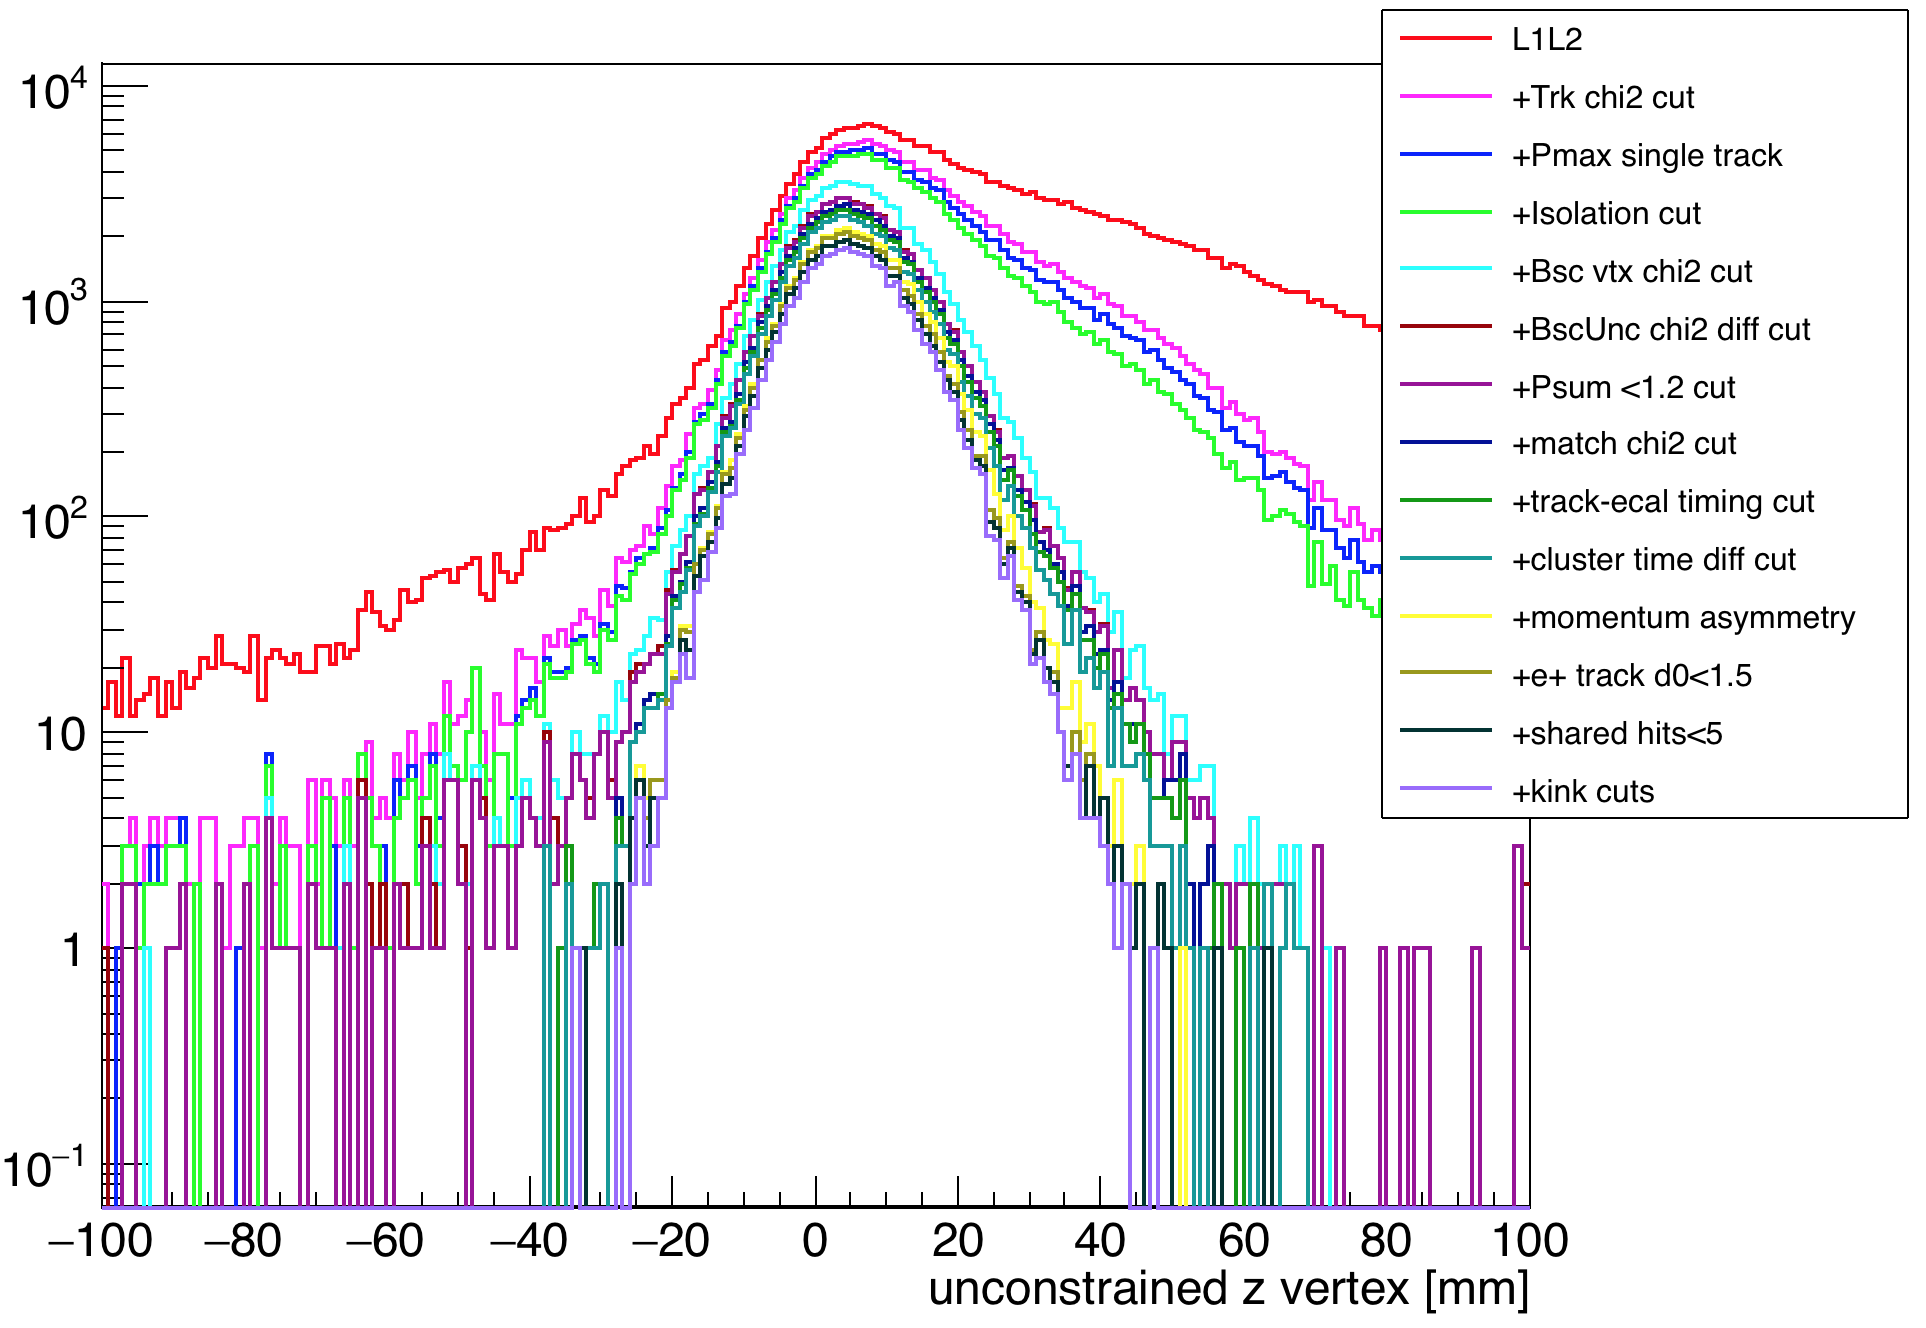
\includegraphics[width=0.8\textwidth]{plots/zvtxCuts_L1L2.png}
  \caption{The effects of the cuts on the L1L2 dataset on the unconstrained z vertex.}
  \label{fig:zvtxCuts_l1l2}
\end{figure} 

The effects of the cuts on the reconstructed mass distribution are shown in Figure~\ref{fig:massCuts_l1l2}.

\begin{figure}[H]
  \centering
      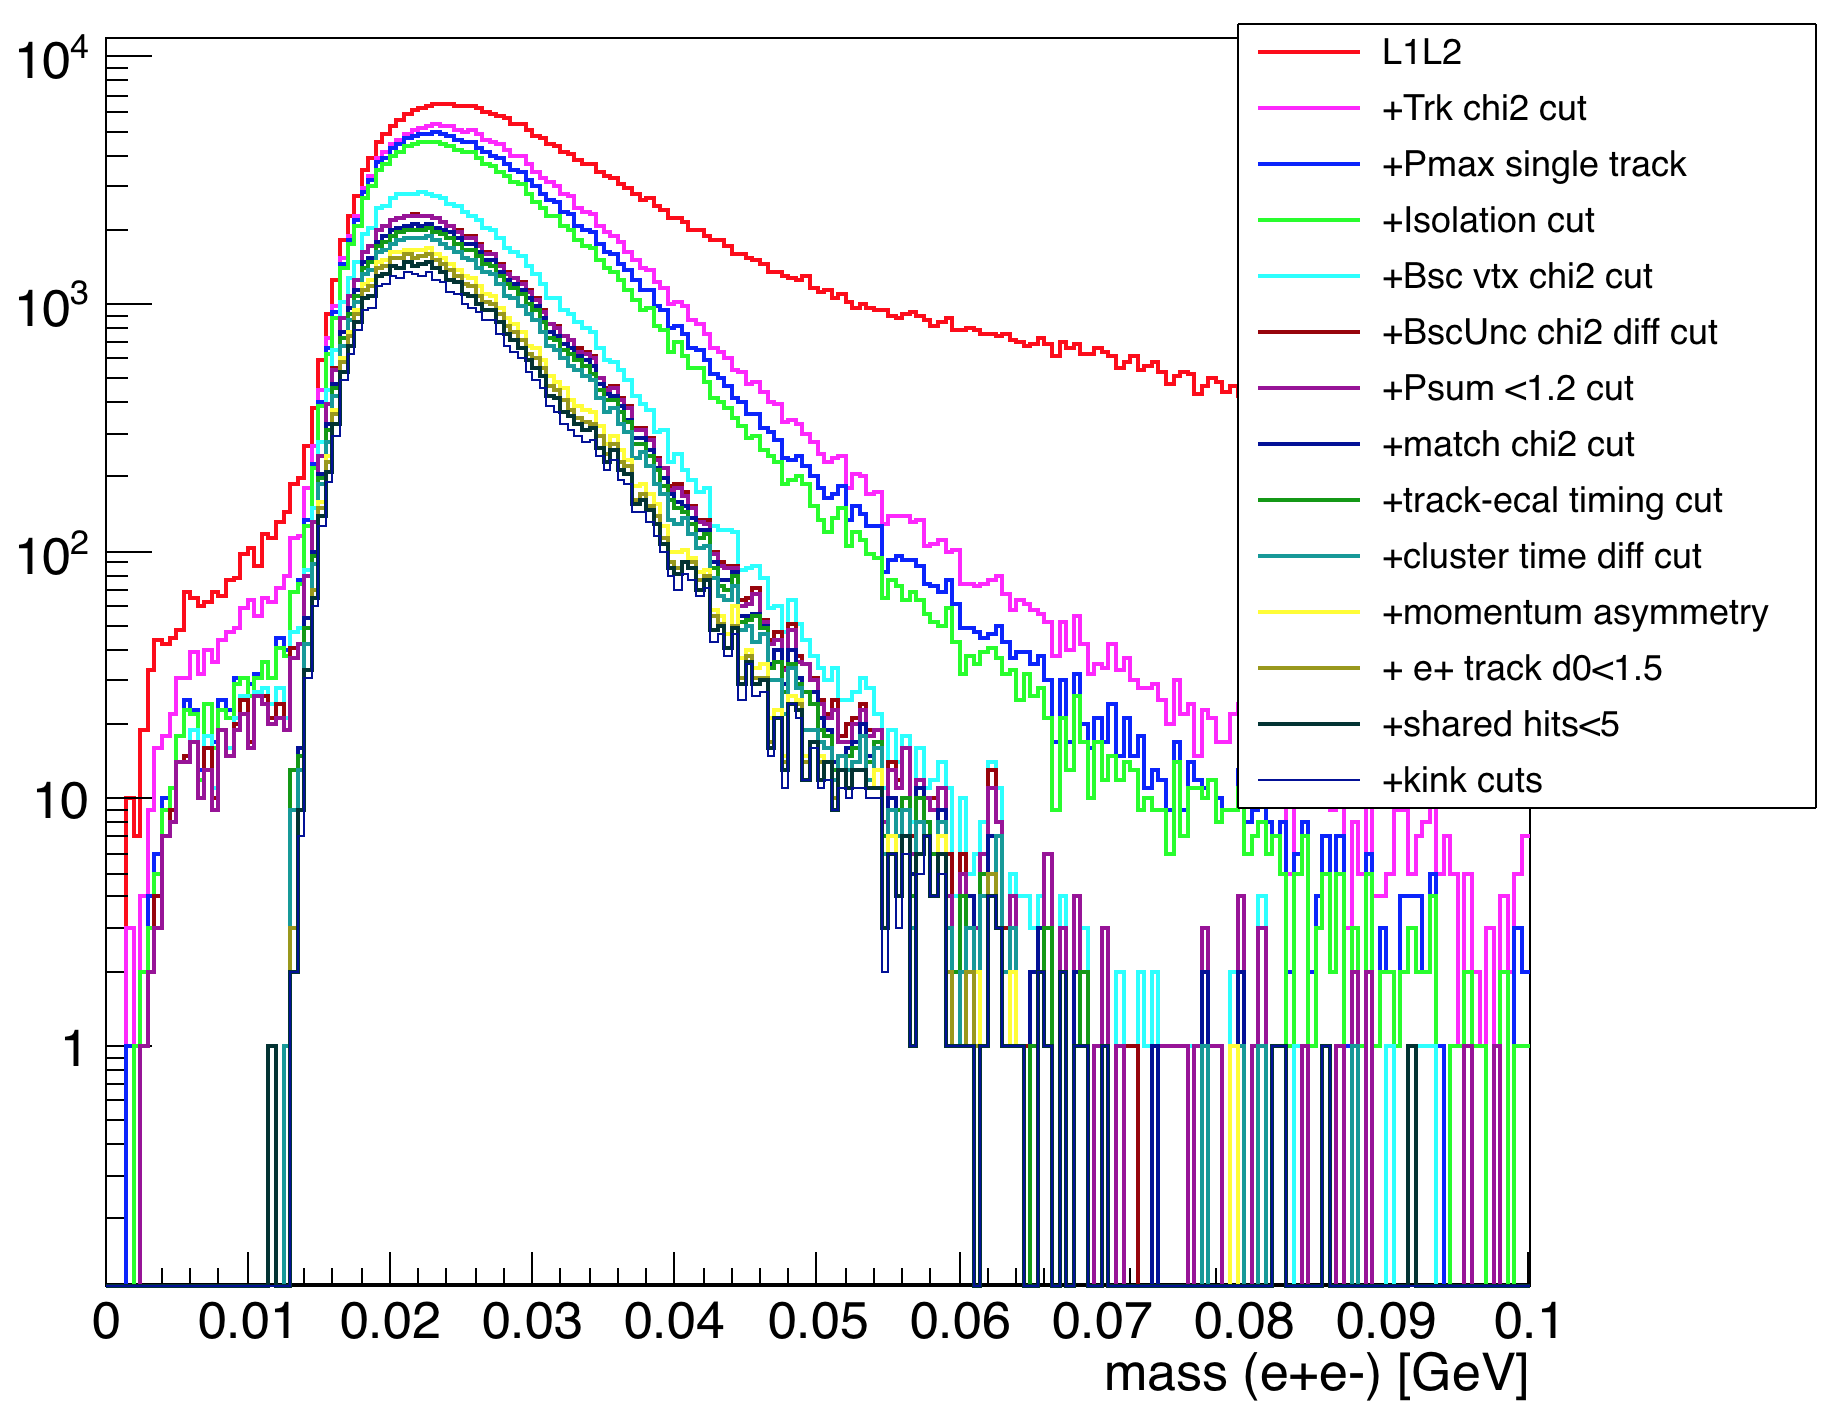
\includegraphics[width=0.8\textwidth]{plots/massCuts_L1L2.png}
  \caption{The effects of the cuts on the L1L2 dataset on the mass distribution.}
  \label{fig:massCuts_l1l2}
\end{figure} 

This dataset has the tendency to contain more WAB contamination than the L1L1 dataset. In particular, we know from Monte Carlo that positrons are unlikely to have a hit in Layer 1 when the photon in WAB pair produces after the target. Additionally, this sample contains a 5:1 ratio of having in electron versus a positron in the first layer. 

\subsubsection{Vertex reconstruction efficiency, $\epsilon_{vtx}$}

The vertex reconstruction efficiency is calculated again as the ratio of reconstructed versus thrown heavy photon Monte Carlo for a range of masses through fixed $\epsilon^{2}$ coupling. As shown in Figure~\ref{fig:apEff}, the reconstructed vertex efficiency as a function of z position can be roughly fit with a Crystal Ball function for events that have any track missing the Layer 1 active region. These efficiencies at each mass are fitted with Equation~\eqref{eq:cbfunction}.


\begin{eqnarray*}
\label{eq:cbfunction}
\epsilon_{vtx}(t >= -| \alpha |) & = & N e^{-0.5t^{2}}\\
\epsilon_{vtx}(t < -| \alpha |) & = & N A(B-t)^{-n}\\
\textsf{where:}\\
\alpha & = & 0.97\\
n & = & 141.5\\
t & = & \dfrac{z-z_{mean}}{\sigma}\\
A & = & (\dfrac{n}{| \alpha |})^{n}e^{-0.5 |\alpha |^2}\\
B & = & \dfrac{n}{| \alpha |}-|\alpha | \\
N & = & \textsf{amplitude of the Gaussian}
\end{eqnarray*}


\begin{equation}
\label{eq:gausfunction}
Ne^{-0.5\dfrac{(z-z_{mean})^2}{\sigma^2}}
\end{equation}

The parameters of the fit are parameterized as  function of mass to find the relations shown in Equation~\eqref{eq:parsEpsVtxL1L2}.

\begin{eqnarray*}
\label{eq:parsEpsVtxL1L2}
z_{mean} & = & -58.89+5208.95m-76469.9m^2+386631m^3\\
\sigma & = & 3.05+629.99m-14691.8m^2+114123m^3\\
N & = & -0.3125+37.0172m-472.052m^2 \\
\end{eqnarray*}

The vertex efficiency for vertices with one track missing Layer 1 can be integrated in accordance with Equation~\eqref{eq:signal}. For a fixed coupling, the integral can be calculated using various zCut values as shown in Figure~\ref{fig:integratedVal2D_l1l2}.

\begin{figure}[H]
  \centering
      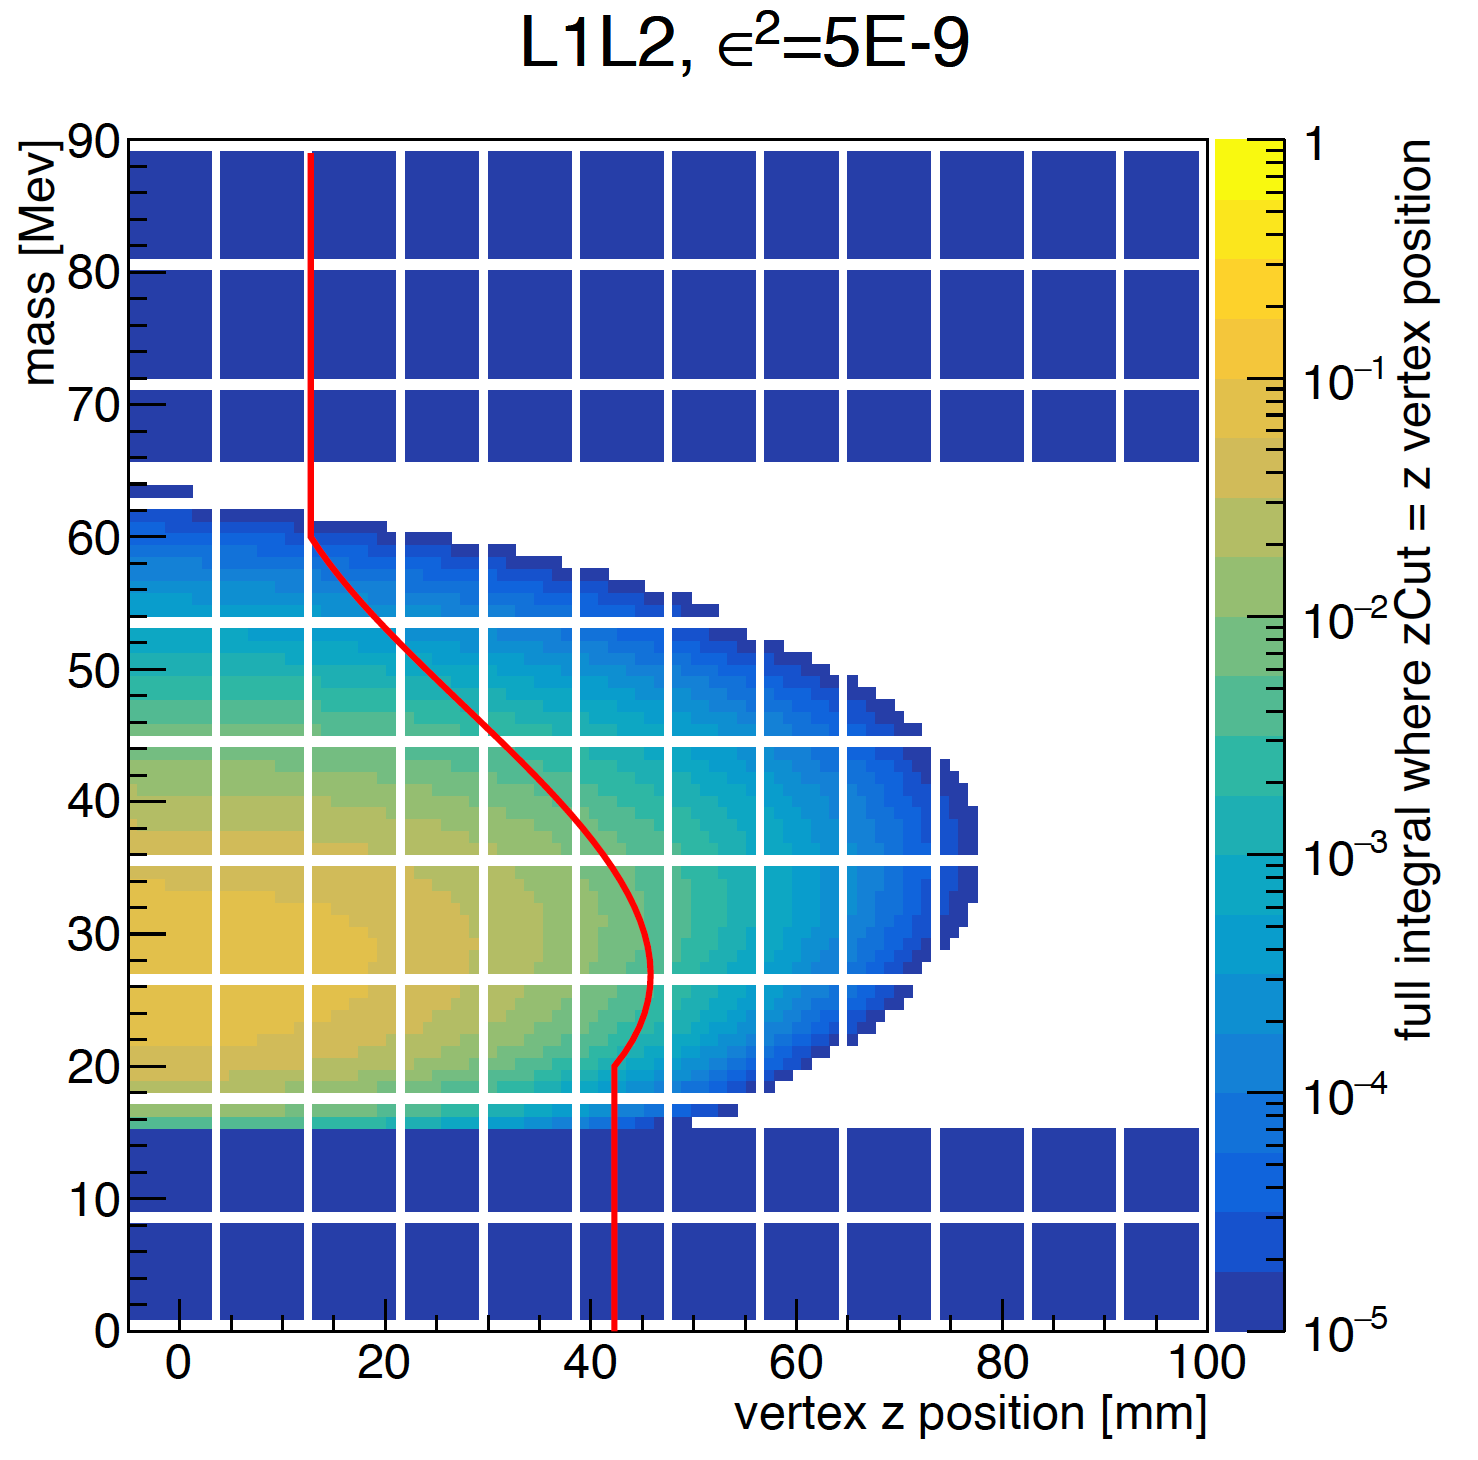
\includegraphics[width=0.8\textwidth]{plots/L1L2_effmz.png}
  \caption{The colored value is the value of the full integral from Equation~\eqref{eq:signal} for the L1L2 dataset using the zCut value on the x-axis. The red line indicates the zCut value derived in data for 0.5 background events. This zCut is drawn from the zCut for the 10~$\%$ unblinded data.}
  \label{fig:integratedVal2D_l1l2}
\end{figure} 

As shown in Figure~\ref{fig:integratedVal2D_l1l2}, the current location of the zCut, if improved by approximately 2-3~mm could improve the reach of the L1L2 dataset.The tails of the z vertex distribution require further studies using the fully unblinded dataset. 


\subsubsection{Mass resolution}

The mass resolution for the L1L2 dataset is obtained by studying A' Monte Carlo, as was the same for the L1L1 dataset. Due to the geometry, the L1L2 dataset improves reach for heavy photons that decay further downstream. The mass resolution is shown in Figure~\ref{fig:massRes_l1l2}.

\begin{figure}[H]
  \centering
      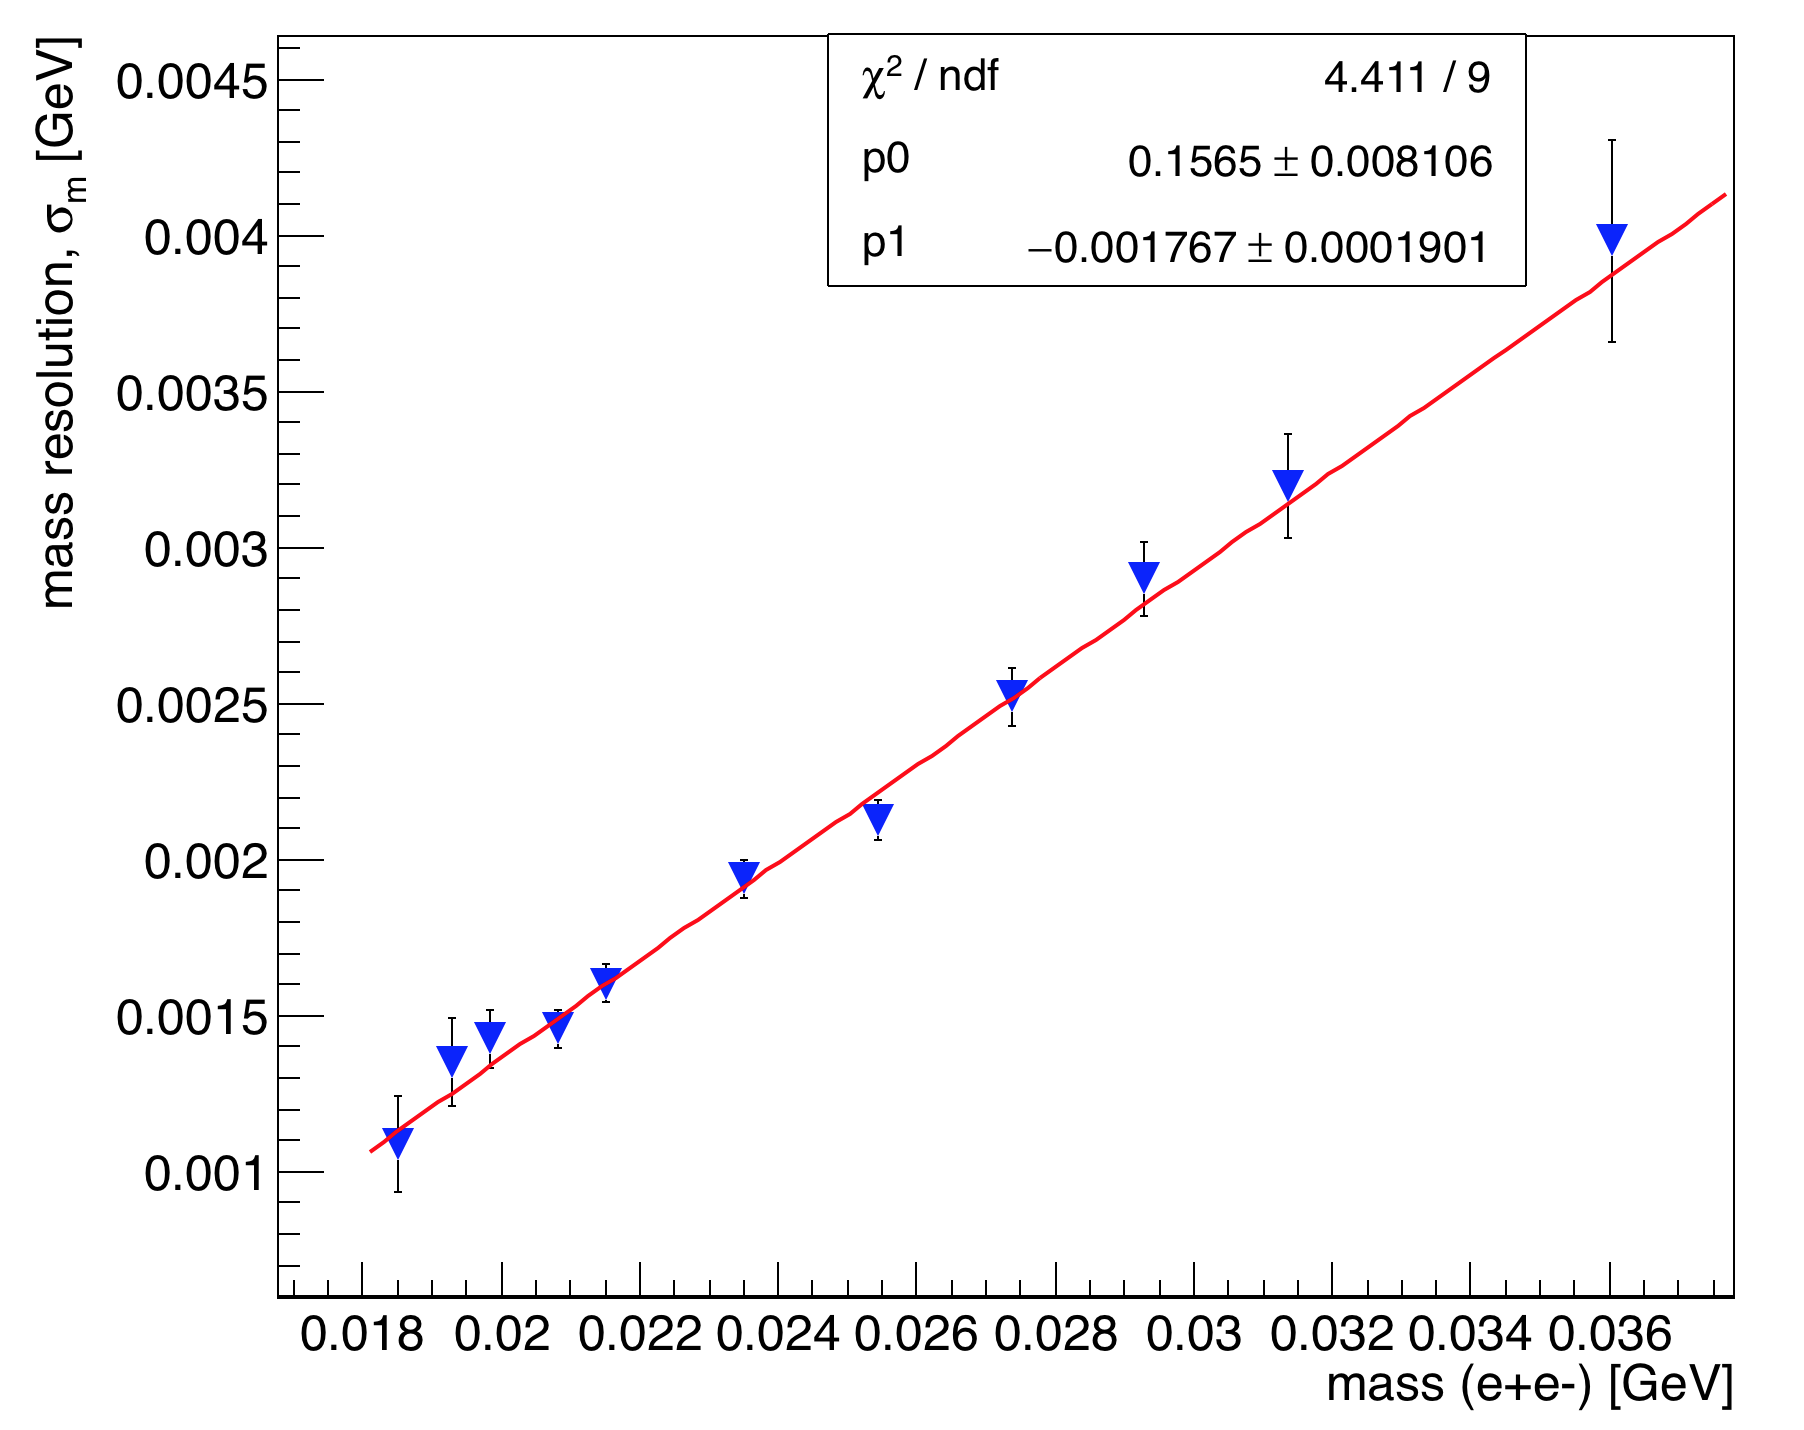
\includegraphics[width=0.8\textwidth]{plots/massRes_L1L2.png}
  \caption{The fitted mass residual, or mass resolution, plotted as a function of the measured mass.}
  \label{fig:massRes_l1l2}
\end{figure} 

The mass resolution for L1L2 decays is noticeably worse than the resolution obtained for the L1L1 dataset.

The fit to the Moller mass distribution in the L1L2 dataset is shown in~\ref{fig:mollerL1L2}.

\begin{figure}[H]
  \centering
      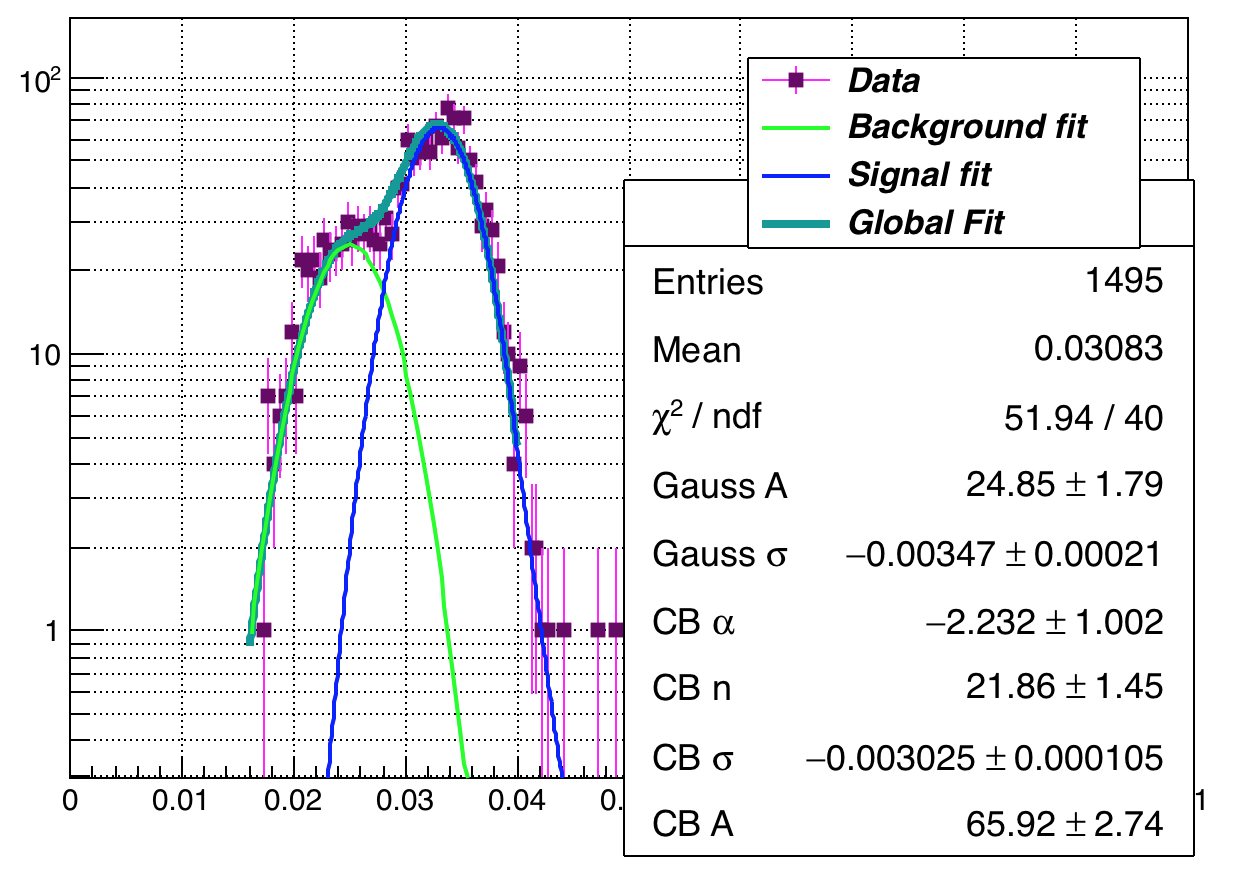
\includegraphics[width=0.8\textwidth]{plots/MollerMassL1L2_data.png}
  \caption{The fit to the L1L2 Moller mass distribution in 10$\%$ of the data.}
  \label{fig:mollerL1L2}
\end{figure} 

The Moller mass peak has a resolution that differs by approximately 2$\%$ with the heavy photon Monte Carlo mass resolution, but the low mass background under the front of the peak is significantly higher than was seen in the L1L1 dataset. This low mass background could be increasing due to the lack of precision without a hit in Layer 1 in tracking and could be responsible for the lack of an apparent mass peak in the L2L2 dataset to be discussed in the next section.

\subsubsection{Accidentals}

The same exercise in studying accidentals in the L1L1 dataset is applied to the L1L2 dataset. By choosing vertices where the time difference between the two clusters is across six beam buckets (time differences greater than 3~ns and less than 9~ns), we observe the vertices produced as a function of mass in Figure~\ref{fig:zVmAcc_l1l2}.

\begin{figure}[H]
  \centering
      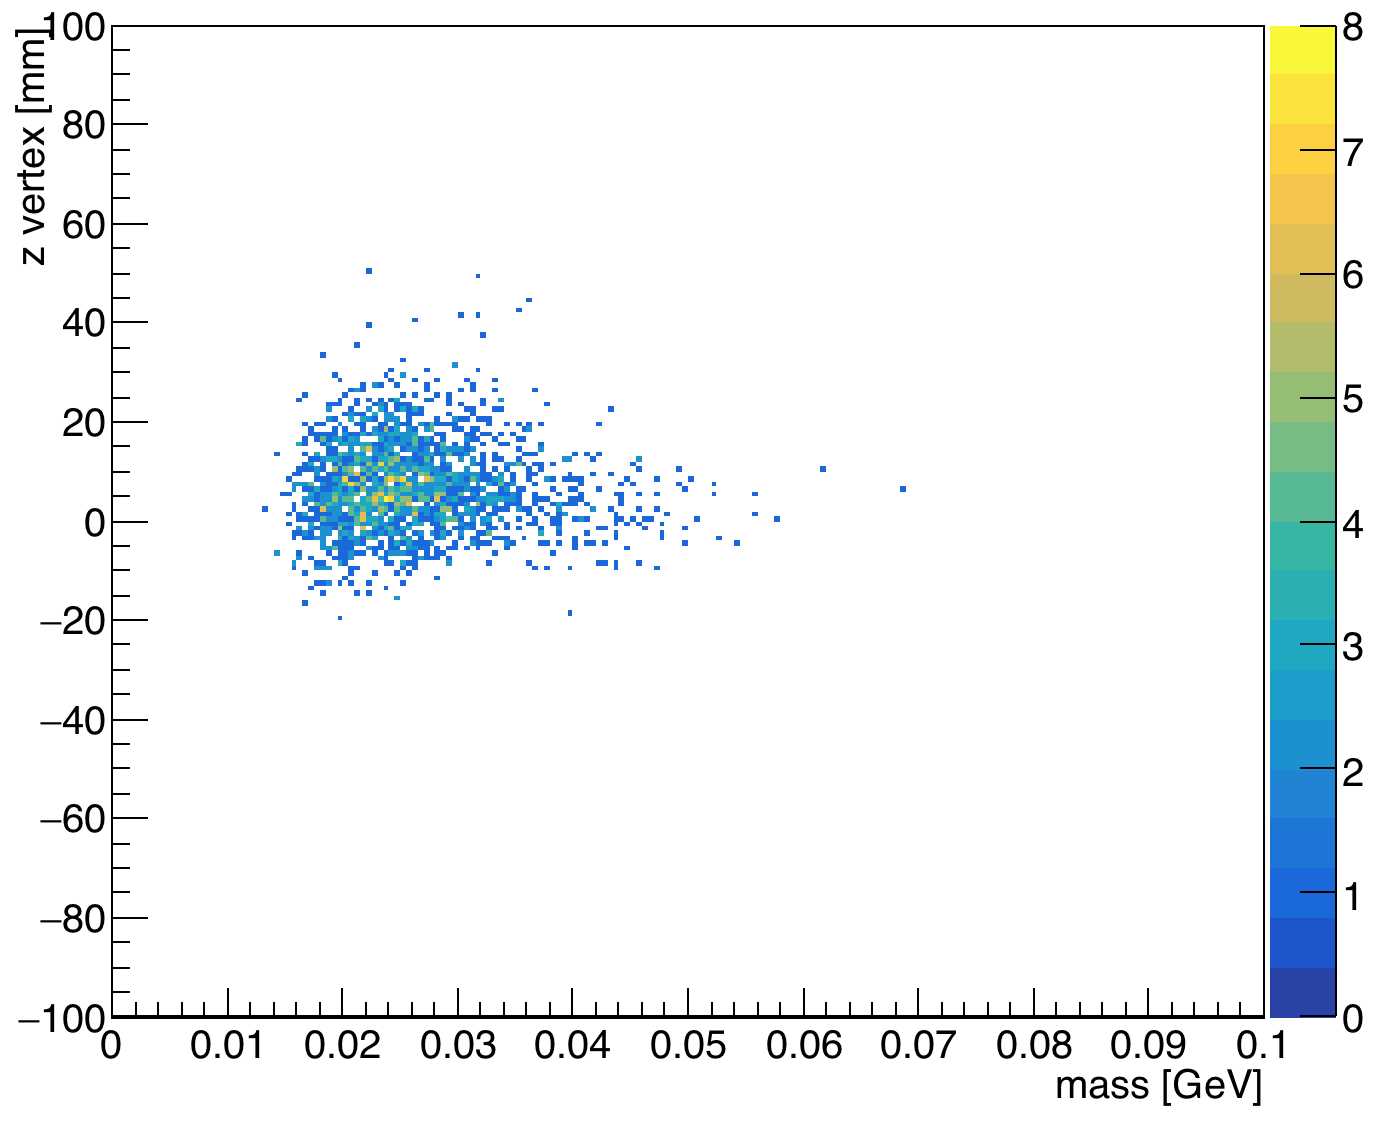
\includegraphics[width=0.8\textwidth]{plots/zVm_acc_L1L2.png}
  \caption{The vertices that are produced when the time difference between the two clusters is greater than 3~ns and less than 6~ns. There are 3 approximately high z background events.}
  \label{fig:zVmAcc_l1l2}
\end{figure} 

As shown in Figure~\ref{fig:zVmAcc_l1l2}, we see that we have obtained approximately 3 high z background events across the six beam buckets. Again, this allows for the possibility to have $1\pm0.6$ background events before in the events selected of the unblinded 10~$\%$ dataset. This rate is seemingly higher than for the L1L1 dataset due to the significantly decreased statistics in the dataset and will require further study with unblinding. 


\subsubsection{Projected reach}

The high z tails of the z vertex distribution as a function of mass can be seen for both datasets where the positron and electron have a Layer 1 hit separately in Figure~\ref{fig:L1L2_datasets}.

\begin{figure}[H]
  \centering
     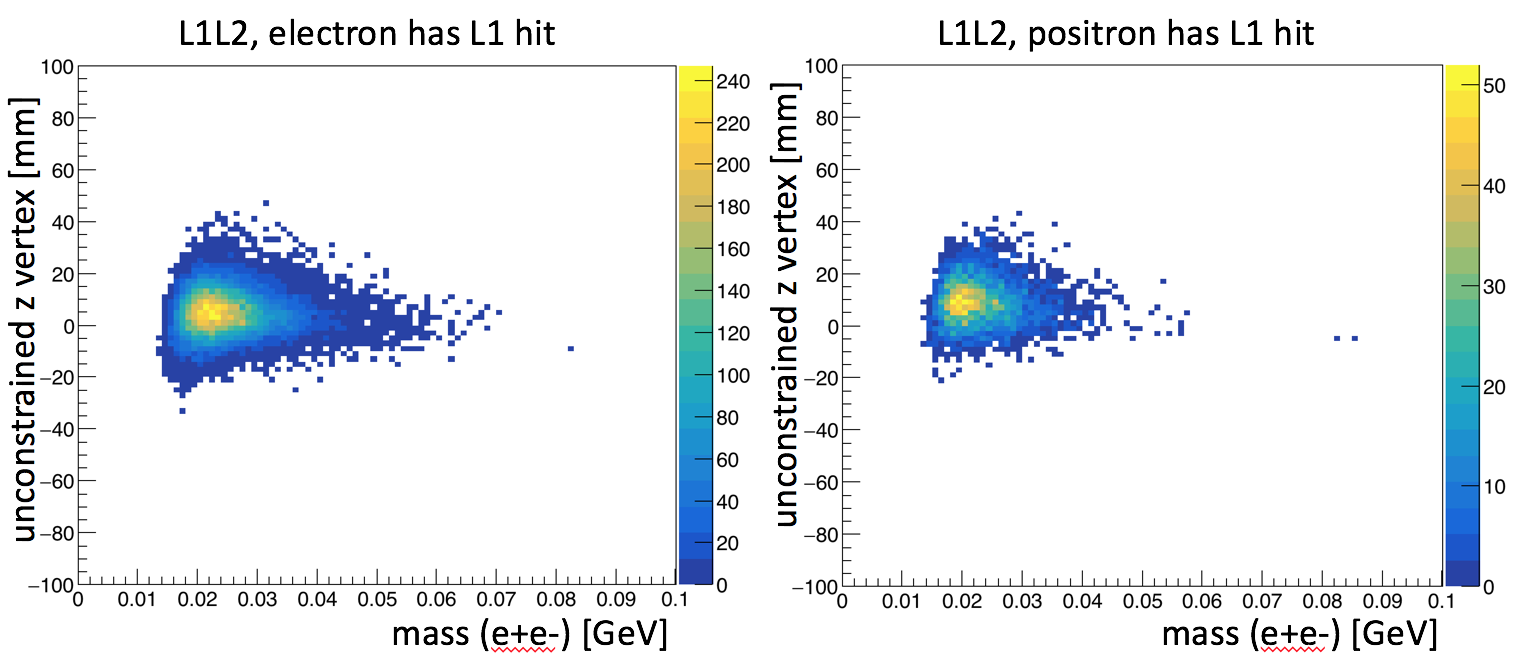
\includegraphics[width=0.8\textwidth]{plots/L1L2_datasets.png}
  \caption{The final z vertex distribution as a function of mass for the L1L2 datasets where the electron has a Layer 1 hit (shown on the left) and the positron has a Layer 1 hit (shown on the right) separately.}
  \label{fig:L1L2_datasets}
\end{figure} 

Because the high z tails for both datasets are similar, the zCut is obtained when we combine these datasets. After unblinding, it could be necessary to tune cuts separately and may merit a separate zCut. For now, the final z vertex distribution as a function of mass can be seen in Figure~\ref{fig:zVm_L1L2}.

\begin{figure}[H]
  \centering
     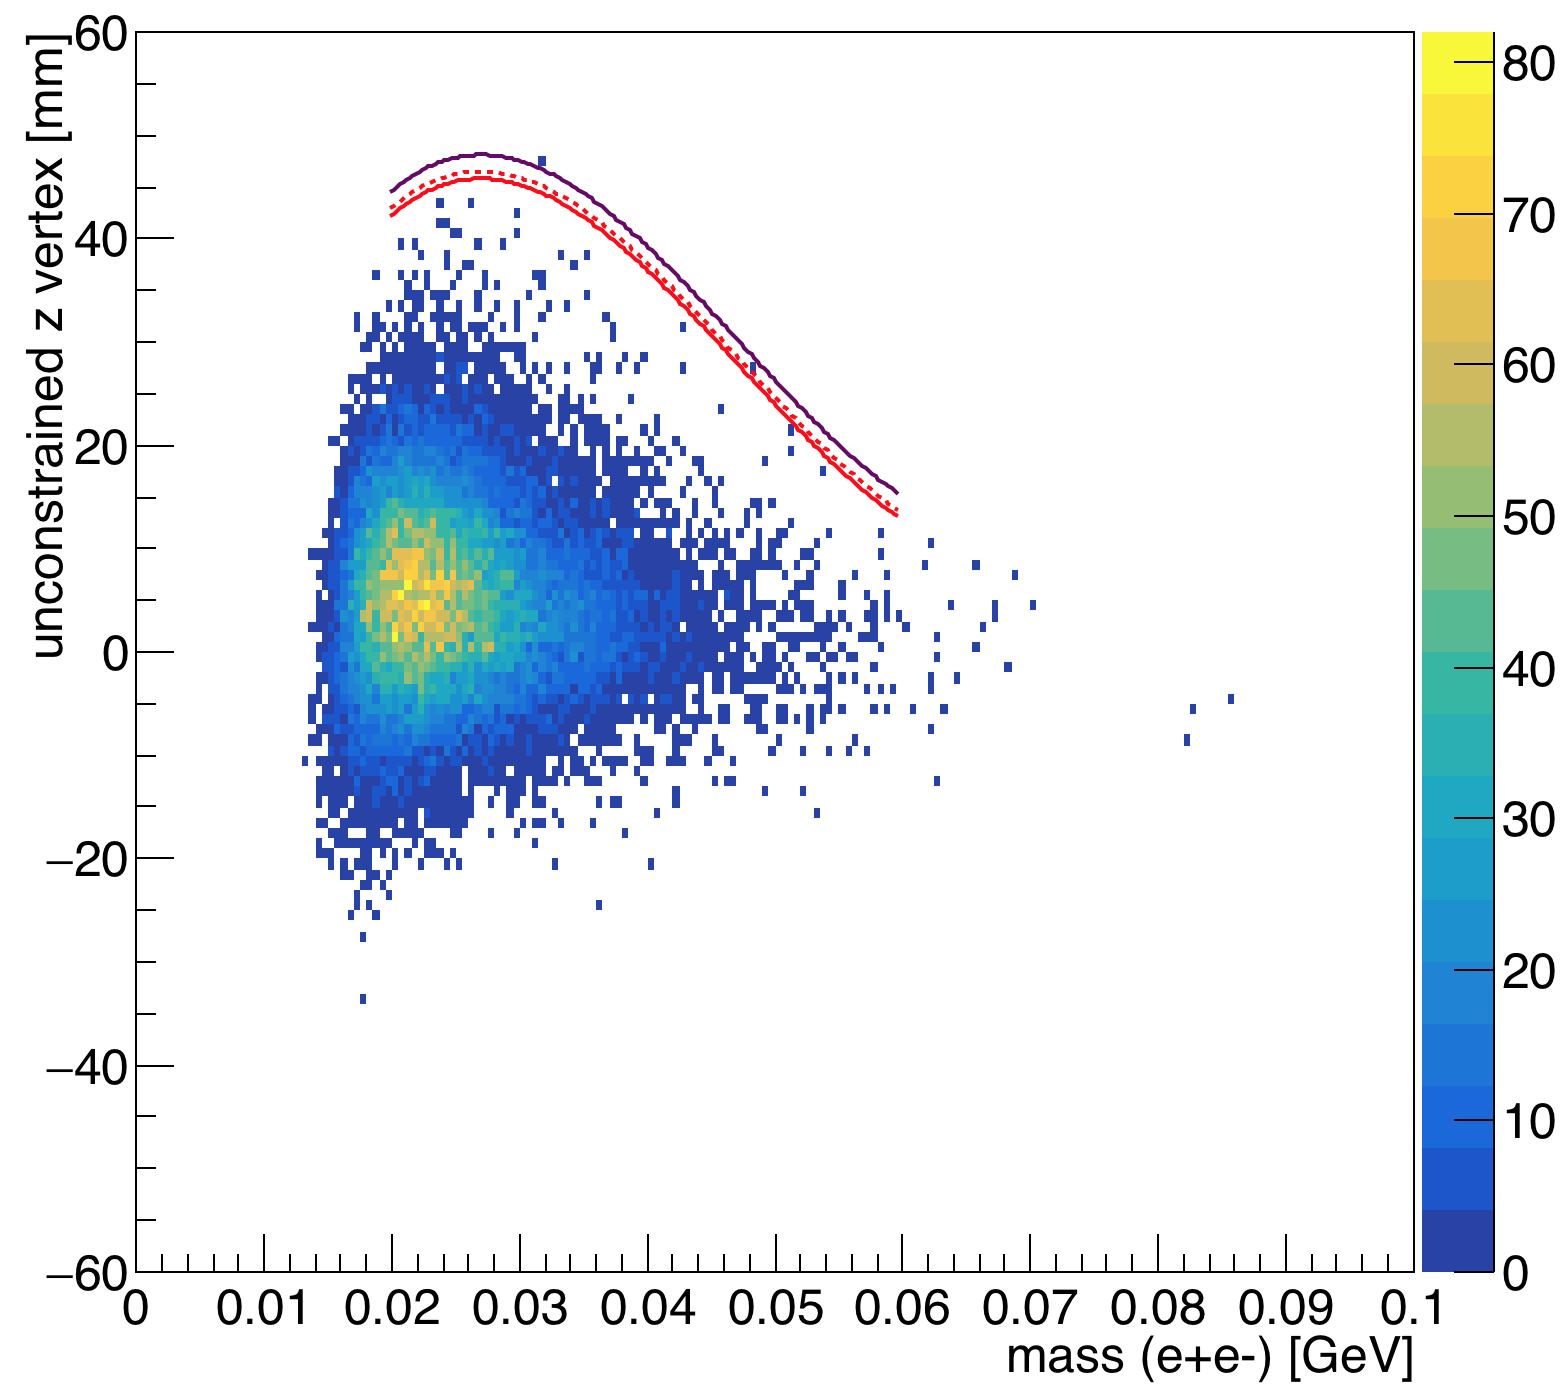
\includegraphics[width=0.8\textwidth]{plots/zVm_L1L2_0p5.png}
  \caption{Reconstructed z vertex as a function of mass for the L1L2 dataset with the first layer of the SVT at 0.5~mm from the beam. The solid red line indicates the zCut found for 10$\%$ of the data (unblinded), and the dashed red line indicates the limit at which events have a quantile greater than 0.5 with respect to the predicted background model. The purple line shows where the projected zCut will be for the full dataset after unblinding.}
  \label{fig:zVm_L1L2}
\end{figure} 

The corresponding reach for the 0.5~mm L1L2 dataset is shown in Figure~\ref{fig:reachl1l2}.

\begin{figure}[H]
  \centering
     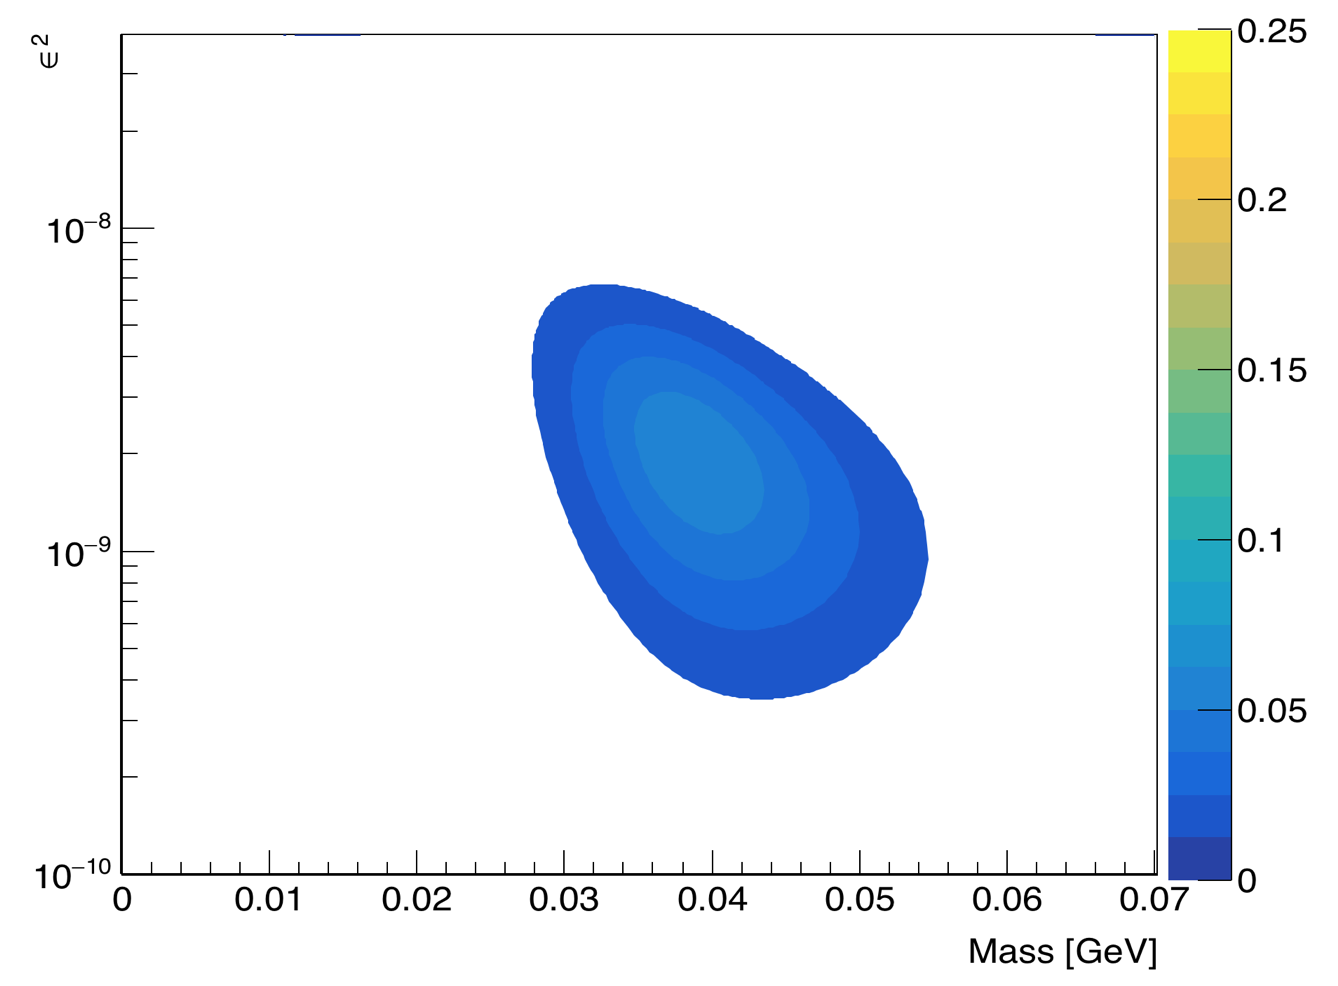
\includegraphics[width=0.8\textwidth]{plots/reachL1L2.png}
  \caption{The expected signal yield for the full 0.5~mm 100$\%$ dataset with L1L2 type events. This uses the zCut projection shown in Figure~\ref{fig:zVm_L1L2}.}
  \label{fig:reachl1l2}
\end{figure} 

The reach distribution for the L1L2 dataset appears to favor weakly coupled larger masses. 
